\documentclass[12pt,openany,a4paper]{book}
\usepackage{graphicx}	% if you want encapsulated PS figures.

% If you use a macro file called macros.tex :
% \input{macros}
% Note: The present document has its macros built in.

% Number subsections but not subsubsections:
\setcounter{secnumdepth}{2}
% Show subsections but not subsubsections in table of contents:
\setcounter{tocdepth}{2}

\pagestyle{headings}		% Chapter on left page, Section on right.
\raggedbottom

\setlength{\topmargin}		{-5mm}  %  25-5 = 20mm
\setlength{\oddsidemargin}	{10mm}  % rhs page inner margin = 25+10mm
\setlength{\evensidemargin}	{0mm}   % lhs page outer margin = 25mm
\setlength{\textwidth}		{150mm} % 35 + 150 + 25 = 210mm
\setlength{\textheight}		{240mm} % 

\renewcommand{\baselinestretch}{1.2}	% Looks like 1.5 spacing.

% Stop figure/tables smaller than 3/4 page from appearing alone on a page:
\renewcommand{\textfraction}{0.25}
\renewcommand{\topfraction}{0.75}
\renewcommand{\bottomfraction}{0.75}
\renewcommand{\floatpagefraction}{0.75}

% THEOREM-LIKE ENVIRONMENTS:
\newtheorem{defn}	{Definition}	% cf. \dfn for cross-referencing
\newtheorem{theorem}	{Theorem}	% cf. \thrm for cross-referencing
\newtheorem{lemma}	{Lemma}		% cf. \lem for cross-referencing

% AIDS TO CROSS-REFERENCING (All take a label as argument):
\newcommand{\eref}[1] {(\ref{#1})}		% (...)
\newcommand{\eq}[1]   {Eq.\,(\ref{#1})}		% Eq.~(...)
\newcommand{\eqs}[2]  {Eqs.~(\ref{#1}) and~(\ref{#2})}
\newcommand{\dfn}[1]  {Definition~\ref{#1}}	% Definition~...
\newcommand{\thrm}[1] {Theorem~\ref{#1}}	% Theorem~...
\newcommand{\lem}[1]  {Lemma~\ref{#1}}		% Lemma~...
\newcommand{\fig}[1]  {Fig.\,\ref{#1}}		% Fig.~...
\newcommand{\tab}[1]  {Table~\ref{#1}}		% Table~...
\newcommand{\chap}[1] {Chapter~\ref{#1}}	% Chapter~...
\newcommand{\secn}[1] {Section~\ref{#1}}	% Section~...
\newcommand{\ssec}[1] {Subsection~\ref{#1}}	% Subsection~...

% AIDS TO FORMATTING:
\newcommand{\teq}[1]	{\mbox{$#1$}}	% in-Text EQuation (unbreakable)
\newcommand{\qed}	{\hspace*{\fill}$\bullet$}	% end of proof

% MATHEMATICAL TEMPLATES:
% Text or math mode:
\newcommand{\half}	{\ensuremath{\frac{1}{2}}}	% one-half
\newcommand{\halftxt}	{\mbox{$\frac{1}{2}$}}	  	% one-half, small
% Math mode only:
% N.B. Parentheses are ROUND; brackets are SQUARE!
\newcommand{\oneon}[1]	{\frac{1}{#1}}		  % reciprocal
\newcommand{\pow}[2]	{\left({#1}\right)^{#2}}  % Parenthesized pOWer
\newcommand{\bow}[2]	{\left[{#1}\right]^{#2}}  % Bracketed pOWer
\newcommand{\evalat}[2]	{\left.{#1}\right|_{#2}}  % EVALuated AT with bar
\newcommand{\bevalat}[2]{\left[{#1}\right]_{#2}}  % Bracketed EVALuated AT
% Total derivatives:
\newcommand{\sdd}[2]	{\frac{d{#1}}{d{#2}}}		    % Short
\newcommand{\sqdd}[2]	{\frac{d^2{#1}}{d{#2}^2}}	    % 2nd ("SQuared")
\newcommand{\ldd}[2]	{\frac{d}{d{#1}}\left({#2}\right)}  % Long paren'ed
\newcommand{\bdd}[2]	{\frac{d}{d{#2}}\left[{#2}\right]}  % long Bracketed
% Partial derivatives (same sequence as for total derivatives):
\newcommand{\sdada}[2]	{\frac{\partial {#1}}{\partial {#2}}}
\newcommand{\sqdada}[2]	{\frac{\partial ^{2}{#1}}{\partial {#2}^{2}}}
\newcommand{\ldada}[2]	{\frac{\partial}{\partial {#1}}\left({#2}\right)}
\newcommand{\bdada}[2]	{\frac{\partial}{\partial {#1}}\left[{#2}\right]}
\newcommand{\da}	{\partial}

% ORDINAL NUMBERS:
\newcommand{\ith}	{\ensuremath{i^{\rm th}}}
\newcommand{\jth}	{\ensuremath{j^{\rm th}}}
\newcommand{\kth}	{\ensuremath{k^{\rm th}}}
\newcommand{\lth}	{\ensuremath{l^{\rm th}}}
\newcommand{\mth}	{\ensuremath{m^{\rm th}}}
\newcommand{\nth}	{\ensuremath{n^{\rm th}}}

% SINUSOIDAL TIME AND SPACE-DEPENDENCY FACTORS:
\newcommand{\ejot}	{\ensuremath{e^{j\omega t}}}
\newcommand{\emjot}	{\ensuremath{e^{-j\omega t}}}

% UNITS (TEXT OR MATH MODE, WITH LEADING PADDING SPACE IF APPLICABLE):
% NB: These have not been tested since being modified for LaTeX2e.
\newcommand{\pack}	{\hspace{-0.08em}}
\newcommand{\Pack}	{\hspace{-0.12em}}
\newcommand{\mA}	{\ensuremath{\rm\,m\pack A}}
\newcommand{\dB}	{\ensuremath{\rm\,d\pack B}}
\newcommand{\dBm}	{\ensuremath{\rm\,d\pack B\pack m}}
\newcommand{\dBW}	{\ensuremath{\rm\,d\pack B\Pack W}}
\newcommand{\uF}	{\ensuremath{\rm\,\mu\pack F}}
\newcommand{\pF}	{\ensuremath{\rm\,p\pack F}}
\newcommand{\nF}	{\ensuremath{\rm\,n\pack F}}
\newcommand{\uH}	{\ensuremath{\rm\,\mu\pack H}}
\newcommand{\mH}	{\ensuremath{\rm\,m\pack H}}
\newcommand{\Hz}	{\ensuremath{\rm\,H\pack z}}
\newcommand{\kHz}	{\ensuremath{\rm\,k\pack H\pack z}}
\newcommand{\MHz}	{\ensuremath{\rm\,M\pack H\pack z}}
\newcommand{\GHz}	{\ensuremath{\rm\,G\pack H\pack z}}
\newcommand{\J}		{\ensuremath{\rm\,J}}
\newcommand{\kg}	{\ensuremath{\rm\,k\pack g}}
\newcommand{\K}		{\ensuremath{\rm\,K}}
\newcommand{\m}		{\ensuremath{\rm\,m}}
\newcommand{\cm}	{\ensuremath{\rm\,cm}}
\newcommand{\km}	{\ensuremath{\rm\,k\pack m}}
\newcommand{\mm}	{\ensuremath{\rm\,m\pack m}}
\newcommand{\nm}	{\ensuremath{\rm\,n\pack m}}
\newcommand{\um}	{\ensuremath{\rm\,\mu m}}
\newcommand{\Np}	{\ensuremath{\rm\,N\pack p}}
\newcommand{\s}		{\ensuremath{\rm\,s}}
\newcommand{\ms}	{\ensuremath{\rm\,m\pack s}}
\newcommand{\us}	{\ensuremath{\rm\,\mu s}}
\newcommand{\V}		{\ensuremath{\rm\,V}}
\newcommand{\mV}	{\ensuremath{\rm\,m\Pack V}}
\newcommand{\W}		{\ensuremath{\rm\,W}}
\newcommand{\mW}	{\ensuremath{\rm\,m\Pack W}}
\newcommand{\ohm}	{\ensuremath{\rm\,\Omega}}
\newcommand{\kohm}	{\ensuremath{\rm\,k\Omega}}
\newcommand{\Mohm}	{\ensuremath{\rm\,M\Omega}}
\newcommand{\degs}	{\ensuremath{\rm^{\circ}}}

% LaTeX run-time type-in command:
%
% \typein{Enter \protect\includeonly{...} command (or just type RETURN):}
%
% Uncommenting this command makes LaTeX prompt you for the \includeonly
% list.  At the prompt
%
%	\@typein=
%
% you type
%
%	\includeonly{chap1,chap2}
%
% to include the files chap1.tex and chap2.tex and omit any others.
% To include every \include file, just hit RETURN.
% If you are running LaTeX from xtexsh, you may need to click the mouse
% in the LaTeX window to position the cursor at the \@typein prompt.

\begin{document}

\frontmatter
% By default, frontmatter has Roman page-numbering (i,ii,...).

\begin{titlepage}
\renewcommand{\baselinestretch}{1.0}

\begin{center}

\begin{figure}
  
\includegraphics[width=\linewidth]{UQLogo.png}
\end{figure}

\vspace*{12mm}
\Huge\bf
		CONNECTING VIRTUAL ROBOTICS\\
		TO AN\\
		EXPERIMENTAL PLATFORM\\
\vspace{20mm}
\large\sl
		by\\
		Callum Rohweder
		\medskip\\
\rm
		School of Information Technology and Electrical Engineering,\\
		The University of Queensland.\\
\vspace{30mm}
		Submitted for the degree of\\
		Bachelor of Engineering
		\smallskip\\
\normalsize
		in the field of Mechatronics
		\medskip\\
\large
		June \& 2018.		
\end{center}
\end{titlepage}

\cleardoublepage

\begin{flushright}
	52 KENNIGO STREET\\
	SPRING HILL, QLD, 4000\\
	Tel.\ 0404 639 174\\
	\medskip
	\today
\end{flushright}
\begin{flushleft}
  Professor Shazia Sadiq\\
  Head of School\\
  School of Information Technology and Electrical Engineering\\
  The University of Queensland\\
  St Lucia, Q 4072\\
  \bigskip\bigskip
  Dear Professor Sadiq,
\end{flushleft}

In accordance with the requirements of the degree of Bachelor of
Engineering in the division of 
Mechatronic Engineering,
I present the
following thesis entitled `Connecting Virtual Robotics To An Experimental Platform`.  This work was performed under the supervision of Dr Surya Singh.\\

I declare that the work submitted in this thesis is my own, except as
acknowledged in the text and footnotes, and has not been previously
submitted for a degree at The University of Queensland or any other
institution.

\begin{flushright}
	Yours sincerely,\\
	\medskip

	\medskip
	Callum Rohweder.
\end{flushright}

\cleardoublepage

\chapter{Acknowledgments}

I specifically would like to thank my fellow students in the school of ITEE for assisting me during this project; for listening to the software issues I faced and giving useful insight and direction.

The product of this thesis was created in complete self-sufficiency, with functionality specified by my supervisor.

Acknowledge your supervisor, preferably with a few short and specific
statements about his/her contribution to the content and direction of
the project.  If you collaborated with another student, acknowledge
your partner's contribution, including any parts of the thesis of
which s/he was the principal author or co-author; this information can
be duplicated in footnotes to the chapters or sections to which your
partner has contributed.  Briefly describe any assistance that you
received from technical or administrative staff.  Support of family
and friends may also be acknowledged, but avoid sentimentality---or
hide it in the dedication.

\cleardoublepage

\chapter{Abstract}

% Notice that all \include files are chapters -- a logical division.
% But not all chapters are \include files; some chapters are short
% enough to be in-lined in the main file.

This document is a skeleton thesis for 4th-year students.  The
printable versions (\texttt{skel.dvi, skel.ps, skel.pdf})
show the structure of a typical thesis with some notes on the content
and purpose of each part.  The notes are meant to be informative but
not necessarily illustrative; for example, this paragraph is not
really an abstract, because it contains information not found
elsewhere in the document.  The \LaTeXe\ source file
(\texttt{skel.tex}) contains some non-printing comments giving
additional information for students who wish to typeset their theses
in \LaTeX.  You can download the source, edit out the unwanted
material, insert your own frontmatter and bibliographic entries, and
in-line or \verb+\include{}+ your own chapter files.  Of course the
content of a particular thesis will influence the form to a large
extent.  Hence this document should not be seen as an attempt to force
every thesis into the same mold.  If in doubt about the structure of
your thesis, seek advice from your supervisor.

\tableofcontents

\listoffigures
\addcontentsline{toc}{chapter}{List of Figures}

\listoftables
\addcontentsline{toc}{chapter}{List of Tables}

% If file los.tex begins with ``\chapter{List of Symbols}'':
% \include{los}

\cleardoublepage

\mainmatter
% By default, mainmatter has Arabic page-numbering (1,2,...).


% Chapters may be \include files, each beginning with a line like
%
%	\chapter{Title of chapter}
%
% e.g. if two chapter files were called intro.tex and theory.tex,
% we would say
%
%	\include{intro}
%	\include{theory}

\chapter{Introduction}
%% Introduction of thesis problem and thesis
Remotely controlling a robot or robotic manipulator is a desirable objective with large complications to still be overcome. It is proposed that doing this through a virtual environment can eliminate collisions or undesirable actions that may incidentally occur due to the nature of long distance control, whilst providing the benefits of virtual simulations. Specifically, this thesis focuses on the development a remote interface to a 'Virtual Robotics Environment Platform', VREP. VREP can be used to simulate robotic arms and processes, and includes the commonly used wheel-chair based Kinova Jaco arm which is available at the University of Queensland. The remote interface, otherwise known as the 'client program' (given that it treats VREP as the server), was designed to take input from a user by either keyboard or joystick, and have the motion played out in VREP, corrected for any obstructions, and then control the movement of the Jaco arm through the Kinova Software Development Kit.

%% Introduction to virtual simuations
In all engineering disciplines, virtual simulations allow one to view and interact with an environment or process in a non-destructive manner. Simulations can provide a realistic rendering of an event, whilst providing further detail into physical phenomena that establish design constraints, and optimization techniques. Robotics makes use of lumped electromechanical components to interact with an environment in a desirable manner. Thus, virtual robotics is a necessary field for growth in engineering, as it allows the testing of interactions with an environment whilst giving unforeseen insight.

%% Introduction to robotics
Companies such as those in manufacturing, technical experts in the fields of medicine and surgery, and persons with disabilities all benefit from the capability of robotic manipulators. In most circumstances it is expected that these manipulators can be controlled by a user in real time, however this ability is restricted by inherent delay in the process of receiving an input, calculating an action, and actuating. Further expectations of robotics include optimality and customisation; where it may be desirable for movements of a robot to minimize the energy used in a given process or a robotic arm to pick up a glass a in a certain manner. This provides interconnected layers of desired functionality for a robot; a layer dedicated to moving the manipulator, a layer designed to create movements that meet the user's needs whilst minimizing design criteria, and a monitoring layer that focuses on aspects such as physical constraints and robotic learning.

%% Introduction to remote robotics
With the invention of the internet to provide long range data-resourcing, came a desire to move the control of manipulators and processes to a remote location. The concept of remote robotics is no different to the typical method of controlling manipulators, an input has a desired output, however at some time in between, data is processed and sent through the internet. Given factors such as time to send, packet loss, processing time, and internet traffic, a significant amount of undesirable delay is added and decreases the satisfaction of real-time control. This produces large complications in areas such as remote robotic surgery, where reaction delay may have harmful effects.

%% Introduction to thesis hypothesis
Virtual robotic environments can simulate the true movements of a manipulator given its physical attributes. VREP in particular can calculate the joint angles required to be able to move the hand from one position to another using a physics engine and accuracy of choice. It is believed that allowing a virtual environment to compute the movements required by a remote user will increase the accuracy in movement and decrease the chance of collision of the physical robot.

%% Introduction to thesis scope
Although this thesis does not go into large detail on the testing of the complete product, remote user to physical robotic arm movement, it does go through the design of the remote interface. The problems faced in controlling a robotic arm, design strategies tested, and the future improvements of the client program are presented. This interface was crucial to the success of the whole system, and it was important to refine before interfacing with a physical arm. Included in this document is:

\begin{itemize}
	\item A comparison of different approaches for moving a robotic arm, along with the calculations and methods for refining accuracy and decreasing processing time.
	\item An overview of VREP, and how its features were used to replicate the true movements of the Jaco arm. This includes a comparison of the available physics engines, the use of PID motor control for arm joints and Inverse Kinematics (IK) functionality. 
	\item Validity of using VREP as a real-time simulation tool, looking into aspects such as rendering delay and communication techniques.
	\item The features included in client program and how its functionality was shaped, and the limitations associated with a real-time program performing large amounts of calculations based off user inputs and a remote server.
	\item An overview of the Jaco Kinova arm and it's software development kit, which can be used to control the Jaco arm from VREP or the client program.


\end{itemize}
% list scope


%% Introduction to thesis objectives
To accomplish the task of remotely controlling the Jaco arm with collision avoidance, the project was broken into four main stages. The long-term objectives to acheive the aforementioned goals, presented in \label{Original Objectives}, are:

\begin{itemize}
	\item to configure the external simulation control of VREP and the Jaco arm within. This included retrieving all of the arm's joint information on start-up, so the correct joints can be referenced during connection. The central purpose of this objective was to achieve control of the arm in simulation, getting it to move its gripper to desired coordinates.
	\item using the information from VREP of the arm, and the current joint angles from the physical Jaco arm using the SDK, achieve movement replication between the the physical and virtual systems. The purpose of this was that it would allow tuning of the VREP simulation to mimic the way the physical arm moves and responds to commands.
	\item with VREP tuned appropriately, allow the movement of the physical arm by controlling movement in the simulation. It was predicted that movement in the simulation would come from keyboard commands or on-screen mouse presses.
	\item detect collision, move objects in the laboratory and interact with the environment in simulation, with the Jaco arm replicating the motion.

\end{itemize}


Due to unforeseen circumstances, the objectives presented in this project changed to focus on the different ways of interacting with the virtual arm through VREP's remote API. It's primary focus is the validity of using a remote client to interact with VREP, and whether a good interface with the aforementioned requirements can be created. The objectives of this thesis were to:

\begin{itemize}
	\item Create a user friendly interface for controlling a robotic arm in VREP, robust to arm location within a scene and mode of the virtual arm (forward kinematics or inverse kinematics modes)
	\item Allow the user to give input types as they desire, such as moving the Jaco arm gripper from point to point, or controlling the joint angles individually; with keyboard input or joystick input.
	\item Experiment with different mathematical solutions and physics engines to achieve accurate and fast movement of the virtual robotic arm
	\item Experiment and outline the different functionality VREP has to offer, which may be utilised in the development of the over-arching objectives.
\end{itemize}

% leading introduction statement
From here, a variety of challenges will be pondered as mathematical formulas are derived to describe the motion of a 6 degree of freedom (DOF) arm, and a remote interface is created for allowing real-time movement within VREP.\\

%% default intro
%The introductory chapter describes the importance of the field and the
%scope and significance of your project.  It usually ends with an
%overview of the remainder of the thesis.%
%
%Notice that Arabic page numbering begins with Chapter 1.  Preceding
%pages (known as ``frontmatter'') have Roman numbering.  The
%\texttt{book} document class in \LaTeX\ follows this numbering
%convention by default (see Lamport~\cite{lamport}, p.\,80).
%%
%%\chapter{Literature review / prior art}
%
%You will need to review previous work in the field, which may include
%books and papers (``literature''), patents and commercial products
%(``prior art''), and earlier work in your Department.  This
%information is usually (but not always) collected in a single chapter,
%whose title should preferably be more specific and interesting than
%the one above.
\chapter{Programming Robots to Move}
%% Go through case studies of how robots have been programmed to move in the past
In order to move a robotic arm, two layers of control are required, the motor position control for each joint, and the system that depicts how much the joints need to change angle when moving from one arm configuration to another. Following are some case studies that present methods of controlling a robotic arm, where the maths behind them are left for the theory section of this report.

\section{MATLAB Toolboxes}
Matlab provides an extraordinary amount of support for calculating the important properties required for the control of a robotic manipulator. Below is a sample of some of the useful libraries available that were, and further could be, beneficial to creating an interface for controlling the virtual Kinova Jaco arm remotely.

\subsection{Robotics Toolbox}
%https://robotacademy.net.au/masterclass/inverse-kinematics-and-robot-motion/?lesson=301
Professor Peter Corke, the Director of the Australian Centre for Robotic Vision (ACRV), has designed a Matlab specific toolbox for computing the mechanics associated with robotic manipulators. Included is easy to use functions for creating robotic arms, and calculating parameters such as forward and inverse kinematics, trajectory generation and control systems for motor control. Within the Queensland University of Technology's Robot Academy is 'Master Classes' on using the toolbox through examples of simple manipulators and the theory behind the complex calculus being performed.\\

There are dozens of object files containing the parameters of robotic manipulators; including the 6 DOF puma560 and limited information on the 6DOF Kinova Jaco arm. The parameters within these files contain the link times of the arm, the Denavit-Hartenberg parameters (DH parameters - theory section of this report), and can contain inertial and angle properties for each link. These properties are helpful in computing the forward kinematics, inverse kinematics, and dynamic equation representing the motion and torques on the arm.

With this, the toolbox allows the viewing of the manipulator in desired angles, the movement of the arm between two desired end-effector positions, and the building of the control system controlling the torque at each motor given the current arm configuration. The latter of which is crucially important in providing accurate control of the arm, in ensuring the appropriate power is provided to all of the joint links as it moves over a given trajectory. Unfortunately, it is extremely difficult to compute, and for each degree of freedom contains 10 constants that need finding; mostly inertia terms which for each link depends on its orientation and position relative to the arm's base; thus relying on all link angles between the base and the link of interest. The mechanics of this is presented in the theory section of the report, but the Robotics Toolbox provides functions which compute the inertial, coriolis and gravitational torques acting on the arm. Professor Corke also provides a method of motor control for each link given the aforementioned parameters are known. The method uses the typical motor position control strategy of a Proportional Derivative Controller (details in the theory section) to compute the required motor torque from the error in angle position and velocity, however also includes a feed-forward component of the calculated disturbance torque due to the coupled dynamics between links. 

\begin{center}
\begin{figure}[htb]
  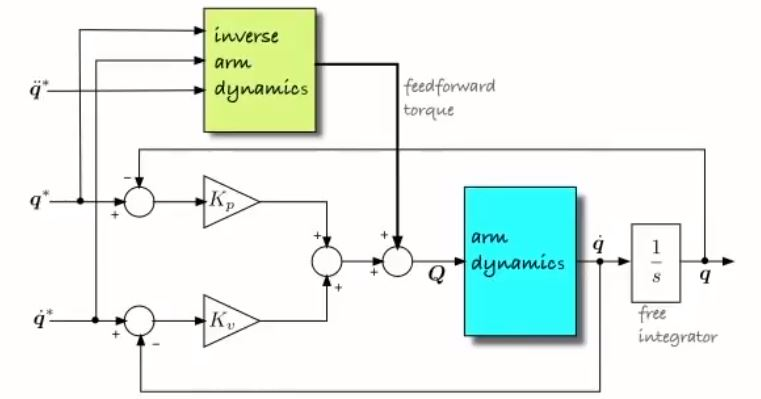
\includegraphics[width=\linewidth]{Correcting_for_disturbance_torque.jpg}
\caption{Motor Torque Control System}
\end{figure}
\end{center}

Thus the torque provided at each link can be expressed as:

$\tau = K_p (q^{*} - q) + K_v (\dot{q^{*}} - \dot{q}) + M(q) \ddot{q^{*}} + C_j (q, \dot{q}) \dot{q} + g_j (q)$

Where the change in angle required by each joint when moving the end-effector from one coordinate to another can be computed using the variation of the 'ikine' function for the given robotic arm; the forward kinematics can be computed similarly using the 'fkine' function.
%% this should be compared to how VREP controls the arm using PID in the theory section. Additionally, the advantage of calculating the dynamic equation for the arm for LQR

\subsection{Robotic Arm Models}
%https://au.mathworks.com/help/physmod/sm/ug/import-robot-arm-model.html
%https://au.mathworks.com/help/control/examples/multi-loop-pid-control-of-a-robot-arm.html?searchHighlight=robotic%20arm&s_tid=doc_srchtitle
Separate to the custom designed toolbox of Professor Corke, MATLAB has its own robot manipulator modelling sub-program and alternative methods of control. Simscape allows the creation of physical systems within MATLAB's simulation tool Simulink. An example of 6 DOF robotic arm is presented below; the base of the arm represents the origin, and the lines span out from this with rigid bodies followed by links. Each rigid body can be shaped within MATLAB or imported from a CAD model to produce a replica of the real robotic arm; where properties such as material and interia can be defined.

\begin{center}
\begin{figure}[htb]
  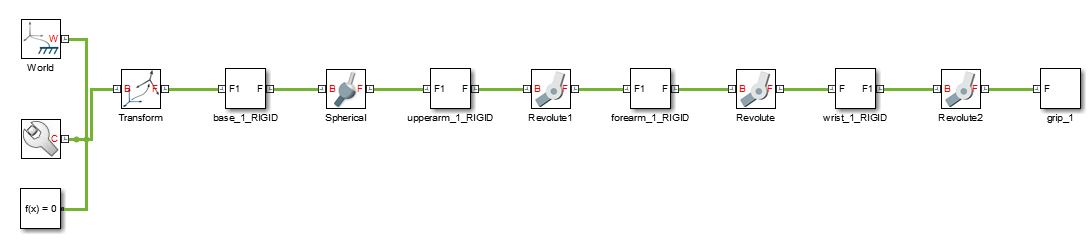
\includegraphics[width=\linewidth]{simscape_robotic_arm.jpg}
\caption{smrobot Simscape Model}
\end{figure}
\end{center}

Simulating the model shown above will provide a visualisation of the arms and any motion set on it by external forces or motor torques; not included in the above model.

\begin{center}
\begin{figure}[htb]
  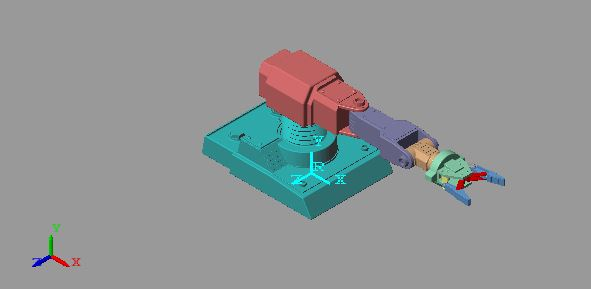
\includegraphics[width=\linewidth]{simscape_robotic_arm_model.jpg}
\caption{smrobot Simscape Model Visualisation}
\end{figure}
\end{center}

From here, it is a matter of controlling the robotic arm to move from one joint configuration to another. For a custom robotic arm, any of the strategies outlined in the theory section of this report can be used, however MATLAB provides another means which is described in the section below. In order to move the joints from one position to the next, a strategy similar to that shown in Figure 2.1 is required. In simulink, the layer of controlling the motor position can be formatted as follows:

\begin{center}
\begin{figure}[htb]
  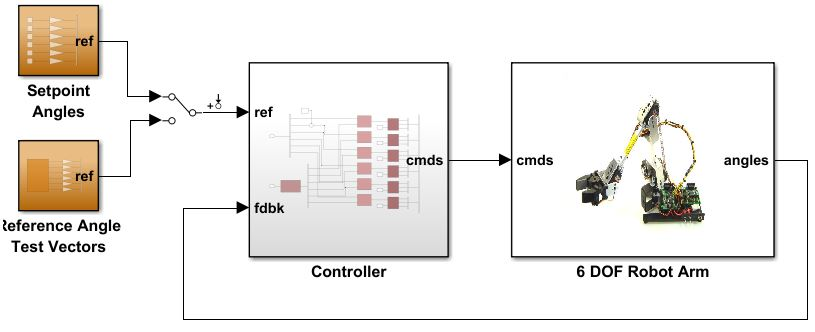
\includegraphics[width=\linewidth]{simulink_motor_control_loop.jpg}
\caption{Simulink Model of Motor Control Loop}
\end{figure}
\end{center}

Where nested within the controller is the tuned PID controllers for each motor which drives it to the desired position. This is similar to Peter Corke's method but without pre-emptive knowledge of the disturbance torque due to the arm's dynamic coupling.

\begin{center}
\begin{figure}[htb]
  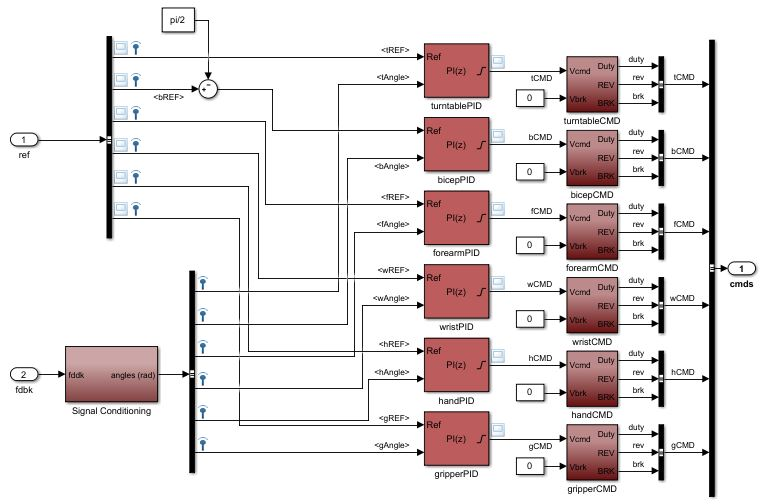
\includegraphics[width=\linewidth]{simulink_motor_control_PID.jpg}
\caption{Simulink Model of Motor Controllers}
\end{figure}
\end{center}

It will be seen that VREP operates in the same way, as it enables the importing of manipulator models and setting of each joint's controller coefficients. The figure above gives a good representation of the mechanics behind what the parameters are doing in terms of regulating each joint's error to a desired angle. A significant advantage of MATLAB is the auto-tuning functionality of the PID controllers for each joint, however a controller on it's own would not be as robust as that described in the Robotics Toolbox section.

\subsection{Adaptive Neuro-Fuzzy Inference System}
%https://au.mathworks.com/help/fuzzy/modeling-inverse-kinematics-in-a-robotic-arm.html?searchHighlight=robotic%20arm&s_tid=doc_srchtitle
An Adaptive Neuro-Fuzzy Inference System (ANFIS) network can be used to deduce the joint angles required for an arm's end-effector to reach a desired 3-D position. Calculating the required angles analytically for an arm of greater than 4 DOF can become challenging and result in infinitely many solutions. Like any neural network, with a sufficiently large dataset the internal weights will learn what angles will result in the desired end-effector position. Thus, in training an ANFIS to control each joint for a training dataset, it is able to interpolate angles to sufficient accuracy and move the joints to reach a desired end-effector position.

To train the network, input to output mapping data is required. Thus, given the forward kinematics for a robotic manipulator is known, a dataset of angles to end-effector position can be created over the space that it is desired for the end-effector to move. After the network gains its own understanding of the mapping, any point within the testing region can be given and the network return the required joint angles. In a MATLAB example, each joint is given its own network to be trained such that for each joint an angle will be provided given a desired position. Outside the range of training, the manipulator will not respond promisingly, and thus for a large control range, a sufficiently large dataset is required. Overall neural networks respond quickly to providing results once trained, however the training process can be time consuming.

\section{Programmed Robotic Arms}


\section{Physics Engines}
\subsection{Bullet Physics Library}

\subsection{Open Dynamics Engine}

\subsection{Vortex Dynamics}

\subsection{Newton Dynamics}



\chapter{Theory}





\subsection{Equations of Motion}



A scientific paper is likely to be read by people who are not
specialists in the same field as the author(s), but who nevertheless
may need to use the results of the paper in their own fields.
Similarly, the examiners of your thesis will probably include at least
one academic who does not teach or conduct research in the subject
area of your thesis.  In an early chapter of your thesis, therefore,
you should quote any theoretical results which are necessary for the
understanding of later chapters.  Examiners who are not specialists in
your area will know whether you have given sufficient theoretical
information.  They will also know whether you have insulted their
status by presenting material which is familiar to every
half-competent graduate in every field of ECE.

\chapter{Methodology, procedure, design, etc.}

This may be one chapter or several.  Again, titles should be more
informative than the above.

You will almost certainly need diagrams to clarify your meaning.  The
\LaTeXe\ \texttt{graphics} package allows the inclusion of PostScript
graphics, as in \fig{flr1}.  The inclusion of \LaTeX\ \texttt{picture}
graphics, as in \fig{fzsys}, requires no auxiliary packages and allows
the mathematical formatting features of \LaTeX\ to be used in
diagrams; but the \texttt{picture} files, unlike PostScript files,
usually require manual editing.





\chapter{Results and discussion \ldots}

\ldots\ or perhaps the discussion should be a separate chapter.

In any case, you will probably need to include tabulated results.
\tab{tf2} illustrates the use of various \LaTeX\ environments to
include a computer printout (plain text file) in a document.  The
\texttt{verbatim} environment, which encloses the formatted text, is
also useful for program listings.

\begin{table}\renewcommand{\baselinestretch}{1.0}
\caption{\sl Fraction of air volume involved in heat exchange for
second mode (right column) vs.\ filling factor (left column).  The
plain-text headings represent $f$, $m$, $\mu_2$ and $f_2$.}
\label{tf2}

\begin{center}
\begin{minipage}[c]{2.85in}\small\normalsize
\begin{verbatim}

 f(%)     m         mu2     f2(%)

 0.016   80.00    0.05400   4.874
 0.031   56.57    0.07732   5.438
 0.062   40.00    0.11103   6.125
 0.125   28.28    0.16001   6.970
 0.250   20.00    0.23175   8.020
 0.500   14.14    0.33799   9.329
 1.000   10.00    0.49789  10.967
 2.000    7.07    0.74444  13.008
 4.000    5.00    1.13919  15.525
 8.000    3.54    1.81095  18.568

19.237    2.28    3.61958  23.174
37.180    1.64    7.28635  27.094
57.392    1.32   14.63631  29.813
74.316    1.16   29.35160  31.453
85.734    1.08   58.79364  32.360
\end{verbatim}
\end{minipage}
\end{center}
\end{table}

\chapter{Conclusions}

\section{Summary and conclusions}

\section{Possible future work}

\appendix

% Chapters after the \appendix command are lettered, not numbered.
% Setting apart the appendices in the table of contents is awkward:

\newpage
\addcontentsline{toc}{part}{Appendices}
\mbox{}
\newpage

% The \mbox{} command between two \newpage commands gives a blank page.
% In the contents, the ``Appendices'' heading is shown as being on this
% blank page, which is the page before the first appendix.  This stops the
% first appendix from be listed ABOVE the word ``Appendices'' in the
% table of contents.

% \include appendix chapters here.

\chapter{Dummy appendix}

Appendices are useful for supplying necessary details or explanations
which do not seem to fit into the main text, perhaps because they are
too long and would distract the reader from the central argument.
Appendices are also used for program listings.

Notice that appendices are ``numbered'' with capital letters, not
numerals.  When the \verb+\appendix+ command in
\LaTeX~\cite[p.\,175]{lamport} is used with the \texttt{book} document
class, it causes subsequent chapters to be treated as appendices.

\chapter{Program listings}

\section{First program}

Some initial explanatory notes may precede the listing.

\section{Second program}

\section{Etc.}

\chapter{Companion disk}

If you wish to make some computer files available to your examiners,
you can list and describe the files here.  The files can be supplied
on a disk and inserted in a pocket fixed to the inside back cover.

The disk will not be needed if you can specify a URL from which the
files can be downloaded.

\cleardoublepage

\begin{thebibliography}{99}
\addcontentsline{toc}{chapter}{Bibliography}
\bibitem{lamport} L.~Lamport, \emph{\LaTeX: A Document Preparation
System}, 2nd ed. (Addison-Wesley, 1994).
\bibitem{LABEL2} REFERENCE 2
\bibitem{ETC.} Etc.
\end{thebibliography}

\end{document}